\section{Coarse spaces}
\begin{frame}{Lid-driven cavity coarse basis functions}
	\begin{figure}
		\centering
		\begin{subfigure}{0.5\textwidth}
			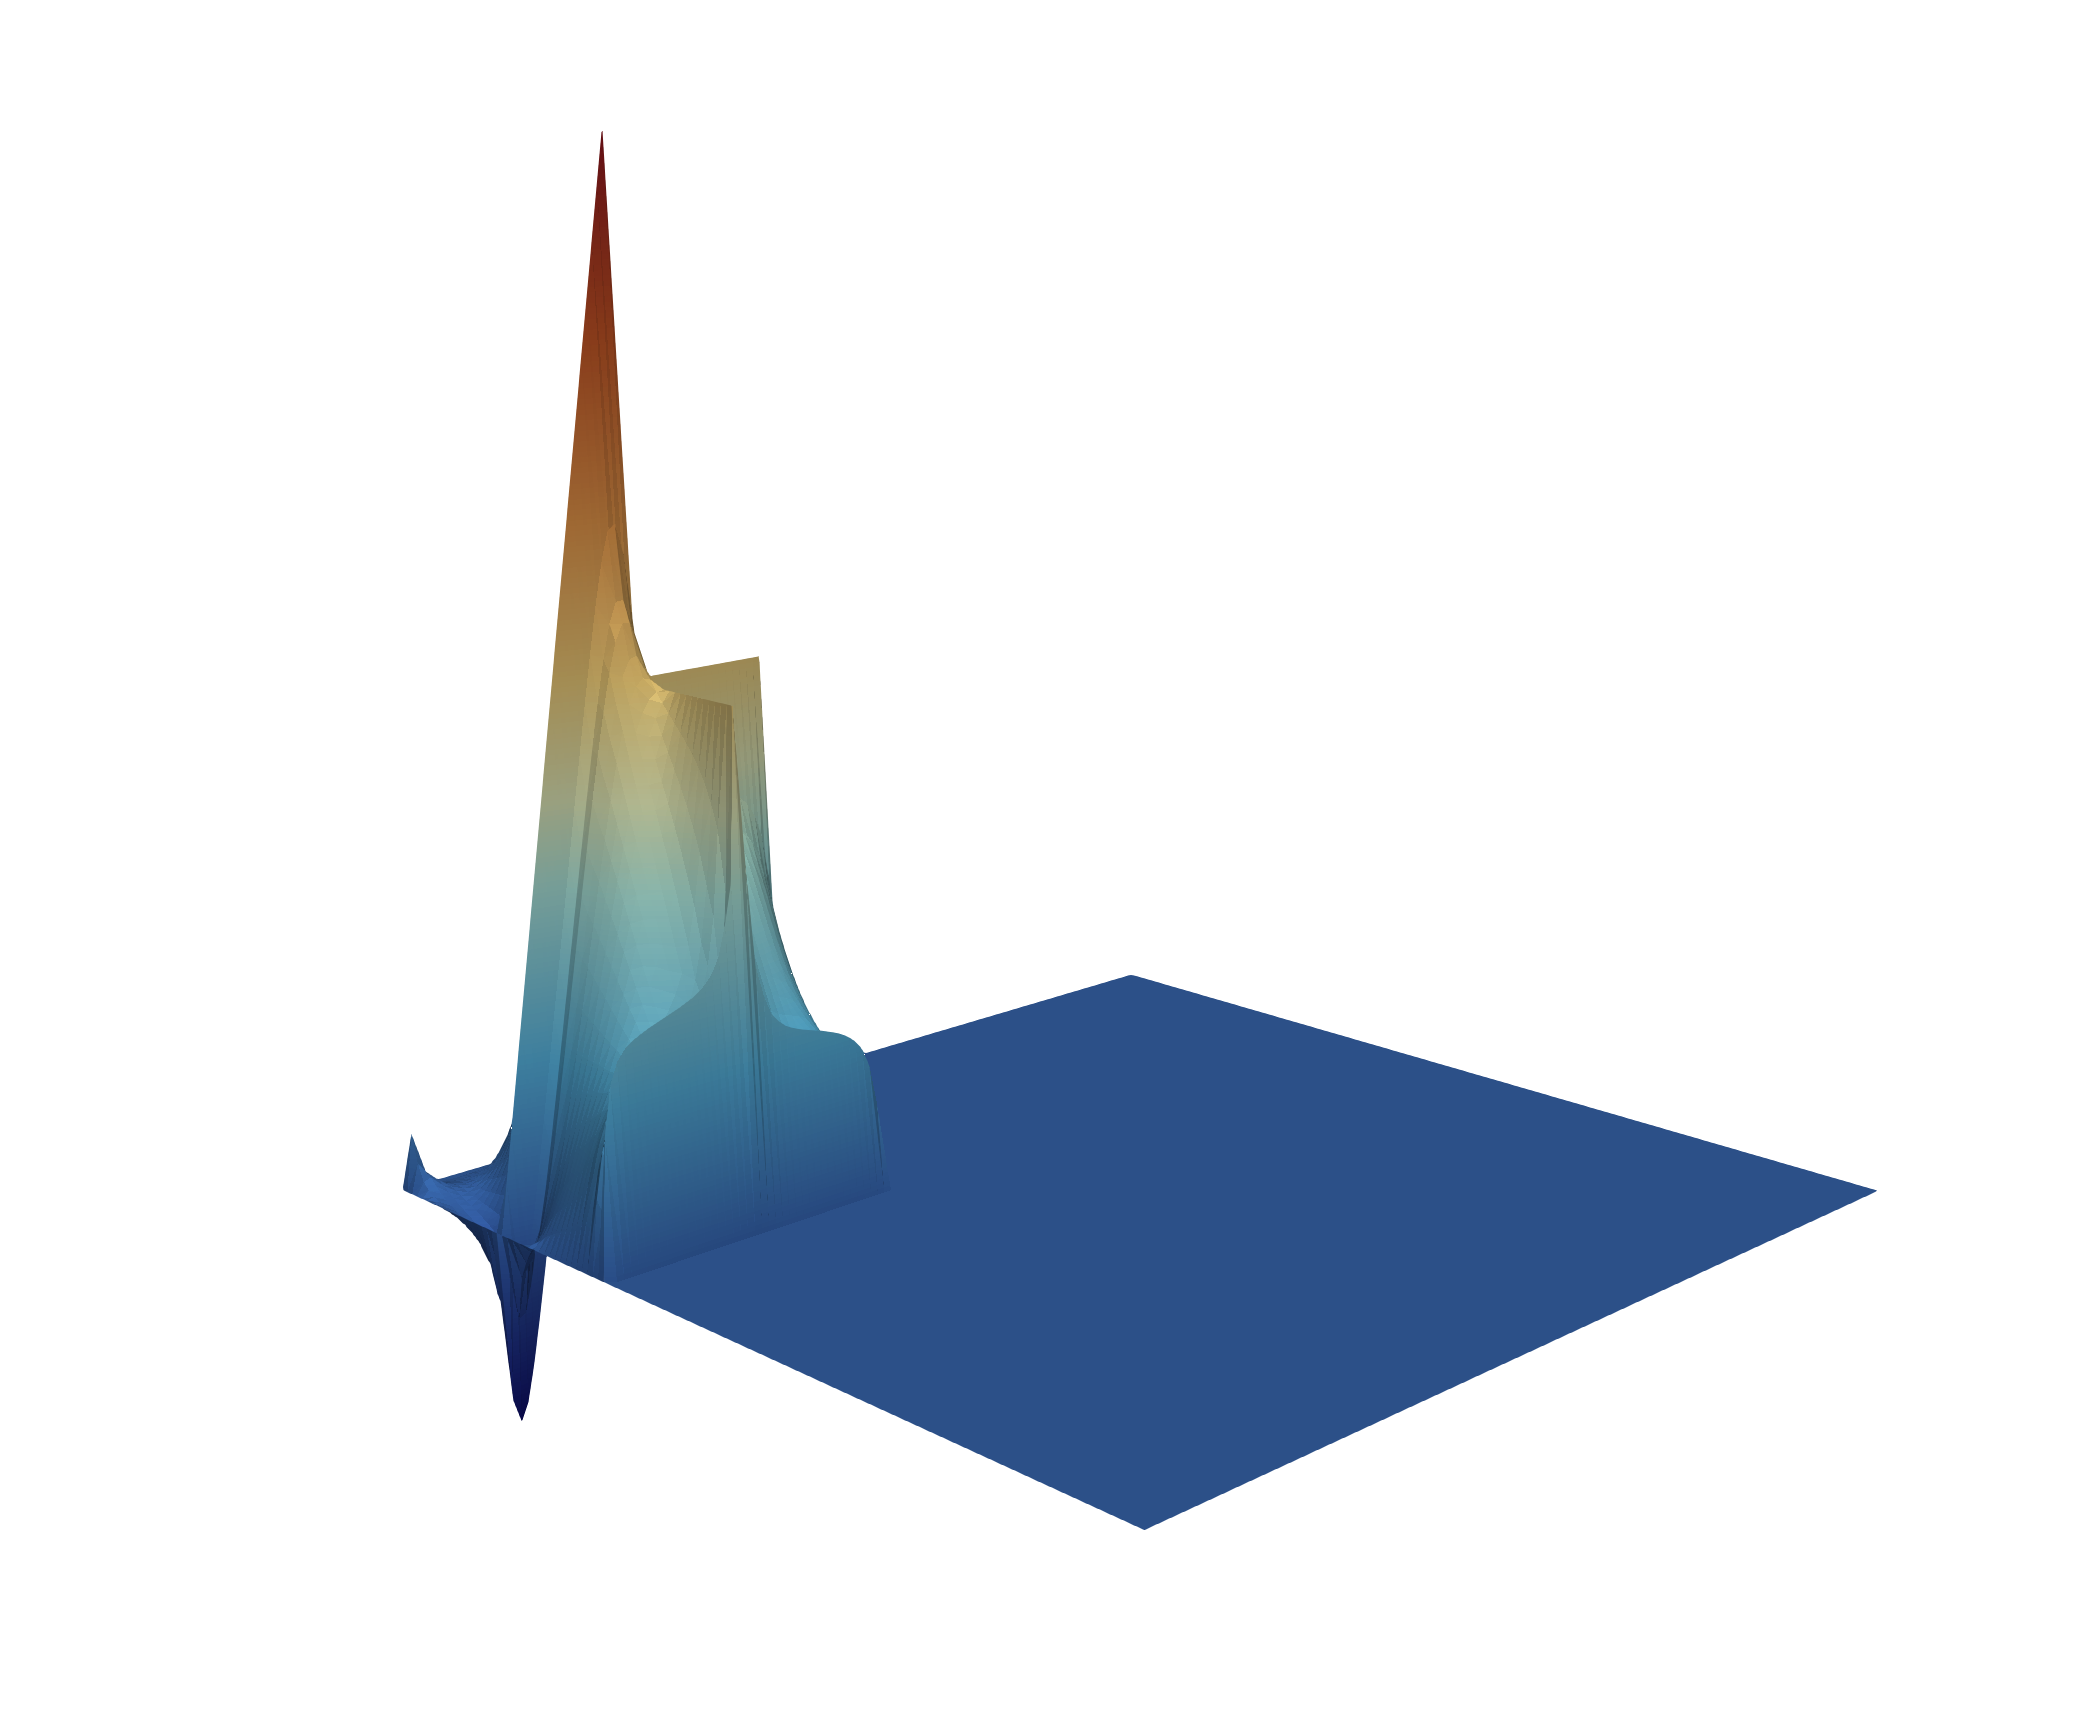
\includegraphics[width=\textwidth]{images/RGDSW-x}
			\caption{RGDSW $x$-component.}
		\end{subfigure}%
		\begin{subfigure}{0.5\textwidth}
			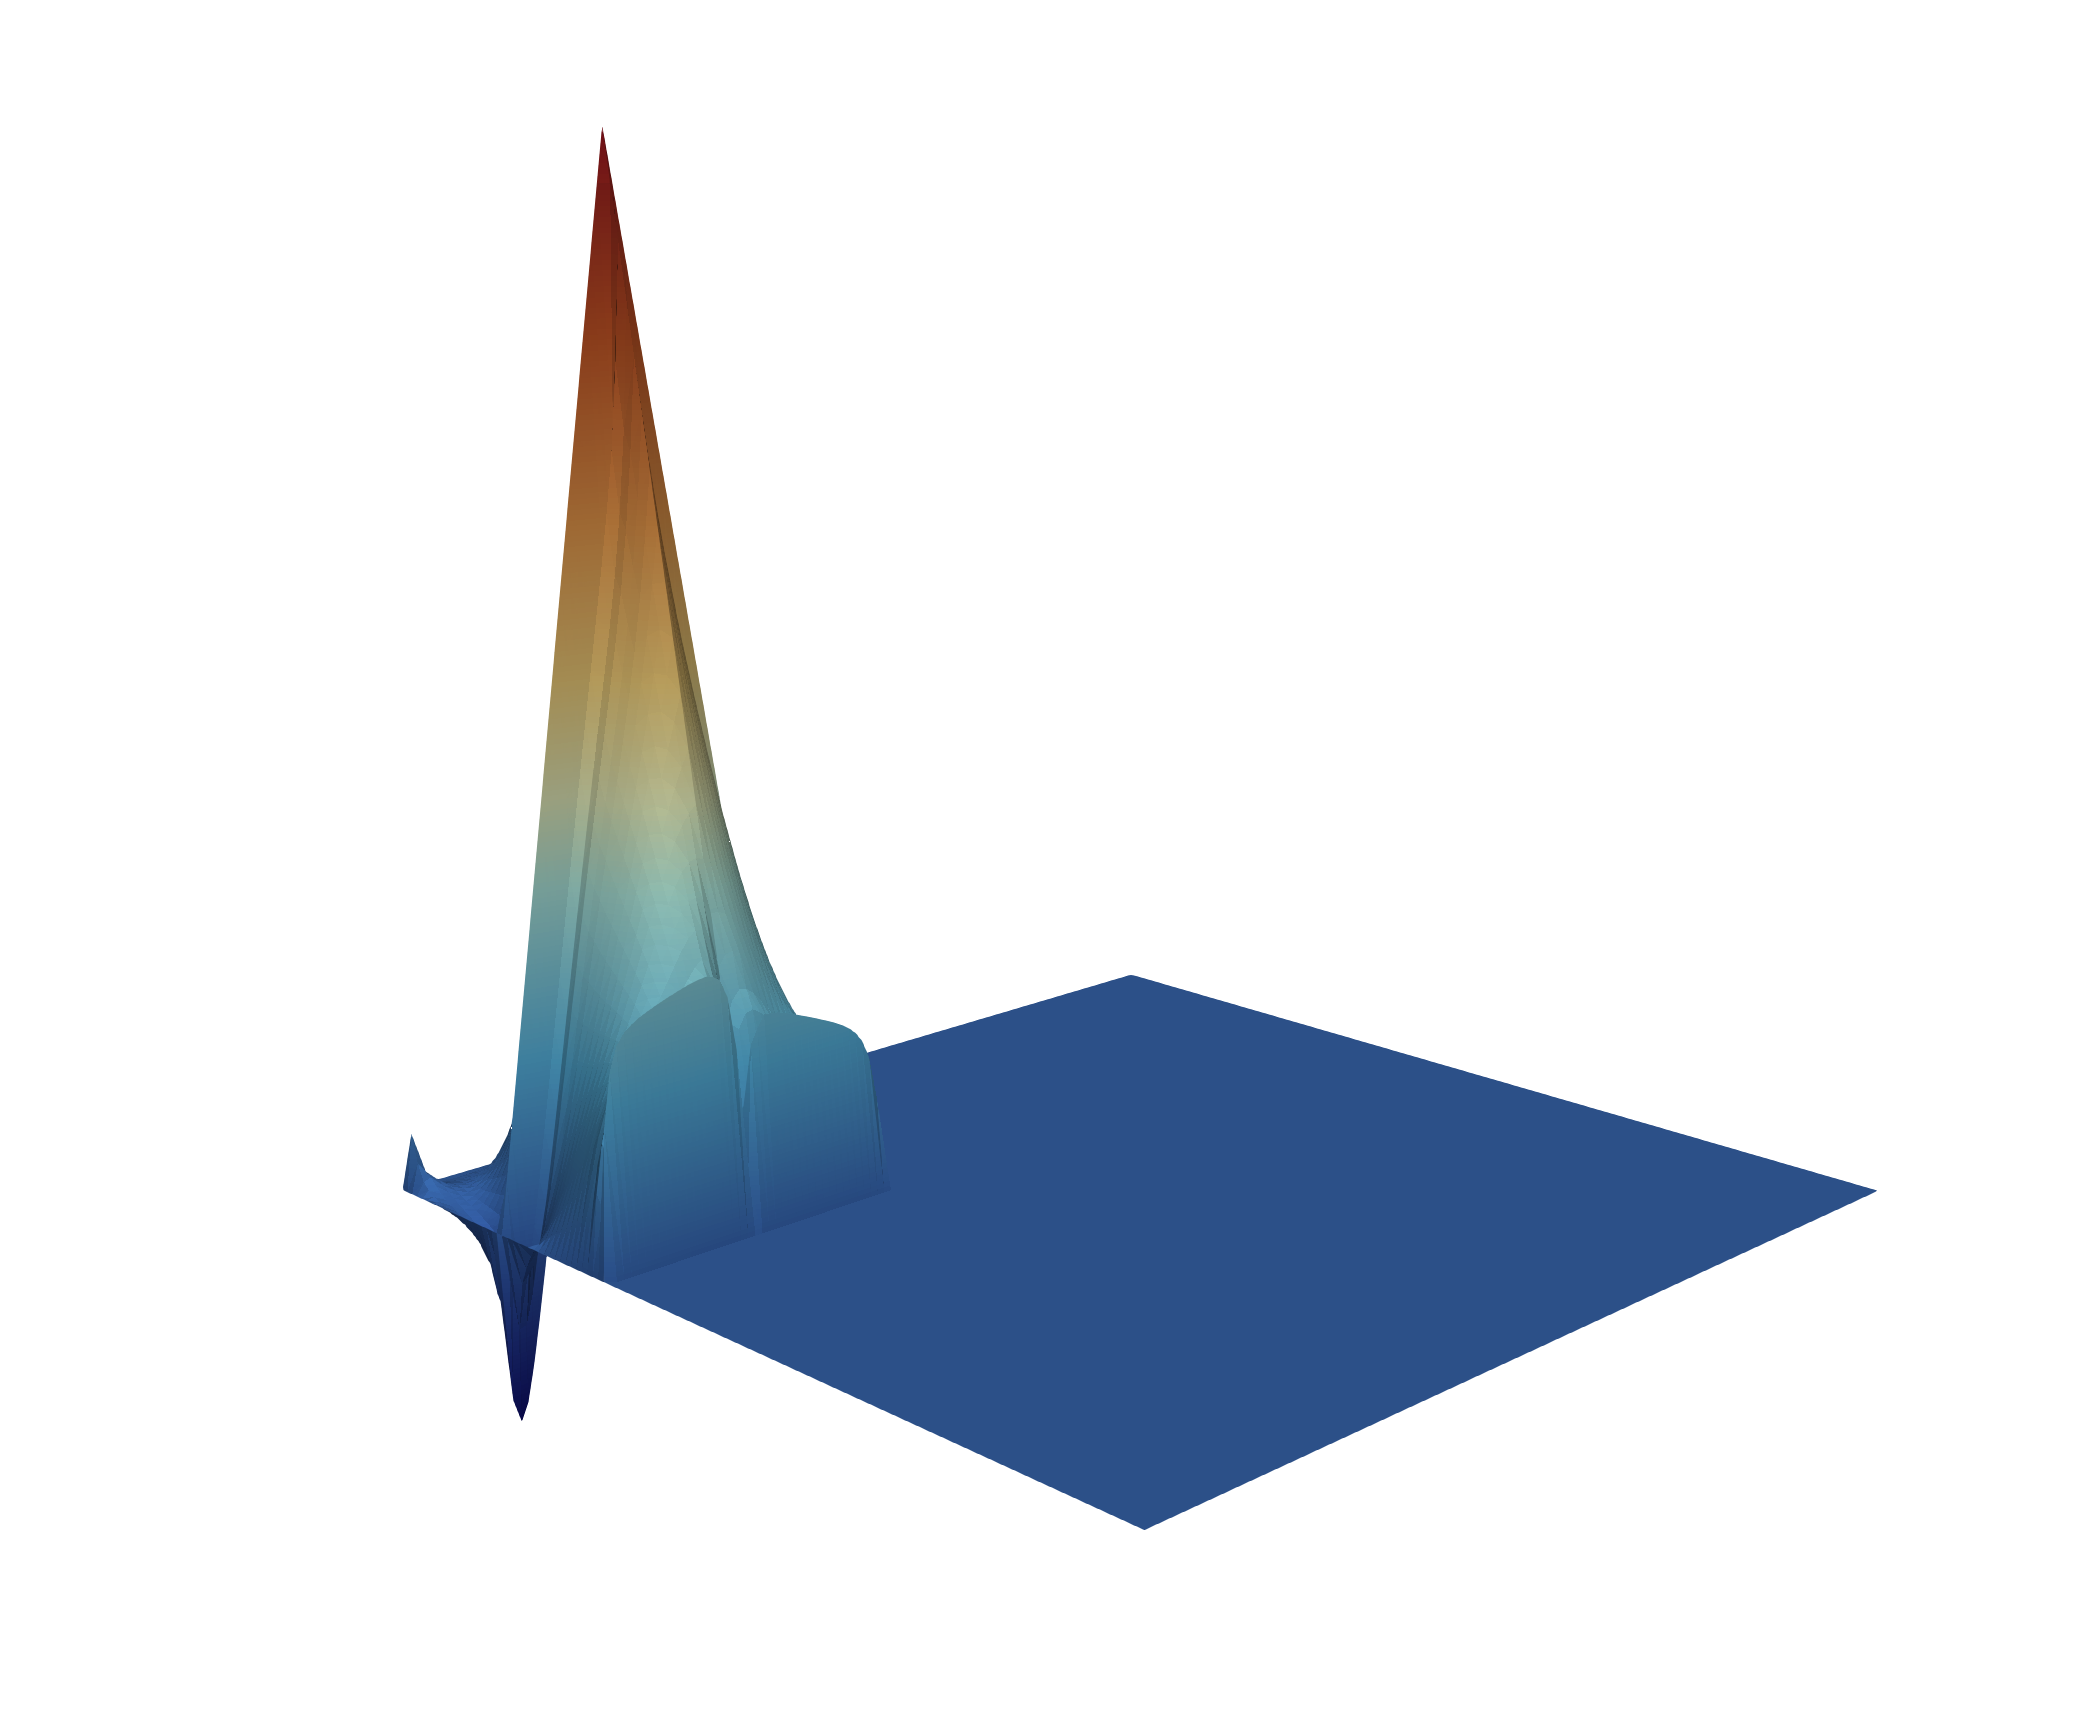
\includegraphics[width=\textwidth]{images/MsFEM-x}
			\caption{MsFEM $x$-component.}
		\end{subfigure}
		\caption{Components of $x$-velocity coarse basis function.}
	\end{figure}
\end{frame}

\begin{frame}{MsFEM vs. RGDSW, 256 subdomains}
	% Mention that: 
	%   - Re has no effect 
	%   - MsFEM was faster for Re=1000 but maybe RGDSW can be sped up with proper tuning
	%   - These results were generated with higher GMRES tollerance which increases GMRES count and runtime without a positive effect
	\begin{figure}
		\centering
		\begin{tikzpicture}
	\pgfplotsset{
		every axis/.append style={
				ybar stacked,
				width=13cm,
				height=7cm,
				ylabel={Runtime (seconds)},
				xlabel={$Re$},
				symbolic x coords={500, 750, 1000, 1500, 2000},
				xtick=data,
				enlarge x limits=0.15,
				legend style={at={(0.9,1)},anchor=north west},
				axis lines*=left, ymajorgrids, yminorgrids,
				ymin=0,
				ymax=175,
				bar width=12pt,
				minor y tick num=1,
				xticklabel style={rotate=0,xshift=0ex,anchor=north},
				cycle list name=Set2-5,
			},
		% Ensures that bars are plotted full
		every axis plot/.append style={
				fill,
			},
	}
	% RGDSW
	\begin{axis}[bar shift=-8pt, hide axis]
		\node [rotate=90](rgdsw) at ([xshift=-8pt]axis cs:500,15) {RGDSW};
		% Inner solve
		\addplot coordinates {(500,22) (750,23.7) (1000,23.8) (1500,31) (2000,0)};
		% Coarse solve
		\addplot coordinates {(500,17.4) (750,17.1) (1000,18.3) (1500,24) (2000,0)};
		% GMRES
		\addplot coordinates {(500,28.6) (750,37) (1000,42.2) (1500,64) (2000,0)};
		% Other
		\addplot coordinates {(500,23.7) (750,22.6) (1000,23.7) (1500,28) (2000,0)};

		\node [rotate=90,anchor=center](500) at ([xshift=-8pt]axis cs:500,105) {$320$ $(4)$};
		\node [rotate=90,anchor=center](750) at ([xshift=-8pt]axis cs:750,113) {$400$ $(4)$};
		\node [rotate=90,anchor=center](1000) at ([xshift=-8pt]axis cs:1000,122) {$450$ $(4)$};
		\node [rotate=90,anchor=center](1500) at ([xshift=-8pt]axis cs:1500,160) {$650$ $(5)$};
		\node at ([xshift=-8pt]axis cs:2000,6) {\scriptsize\color{red}\ding{55}};

	\end{axis}

	\begin{axis}[bar shift=8pt]
		\node [rotate=90](msfem) at ([xshift=8pt]axis cs:500,15) {MsFEM};
		% Inner solve
		\addplot coordinates {(500,21.9) (750,21.9) (1000,0) (1500,0) (2000,0)};
		% Coarse solve                            
		\addplot coordinates {(500,22.3) (750,24  ) (1000,0) (1500,0) (2000,0)};
		% GMRES                                   
		\addplot coordinates {(500,25.6) (750,28.9) (1000,0) (1500,0) (2000,0)};
		% Other                                   
		\addplot coordinates {(500,23.7) (750,23.9) (1000,0) (1500,0) (2000,0)};


		\legend{
			Inner solve,
			Coarse solve,
			GMRES,
			Other
		}
		\node[rotate=90,anchor=center](one) at ([xshift=8pt]axis cs:500,107) {$300$ $(4)$};
		\node[rotate=90,anchor=center] at ([xshift=8pt]axis cs:750,112) {$330$ $(4)$};

		\node at ([xshift=8pt]axis cs:1000,6) {\scriptsize\color{red}\ding{55}};
		\node at ([xshift=8pt]axis cs:1500,6) {\scriptsize\color{red}\ding{55}};
		\node at ([xshift=8pt]axis cs:2000,6) {\scriptsize\color{red}\ding{55}};


	\end{axis}

	\node[rotate=0, text width=1.6cm] (gmres) at ([xshift=8,yshift=40]500){GMRES its. (Newton its.)};
	% \node[rotate=0, text width=1.8cm] (coarsespace) at ([yshift=-60,xshift=-10]1000){Coarse space};

	\draw [thin] (gmres) --  (500);
	\draw [thin] (gmres) --  (one);

	% \draw [thin] (coarsespace) --  (rgdsw);
	% \draw [thin] (coarsespace) --  (msfem);

\end{tikzpicture}

		\label{fig:msfem-vs-rgdsw}
	\end{figure}
\end{frame}

\begin{frame}{Hyperelasticity coarse basis modification}
	\centering
	\vspace{10mm}
	\only<1>{
		\begin{tikzpicture}
	\node[anchor=north west] (main) at (0, 0) {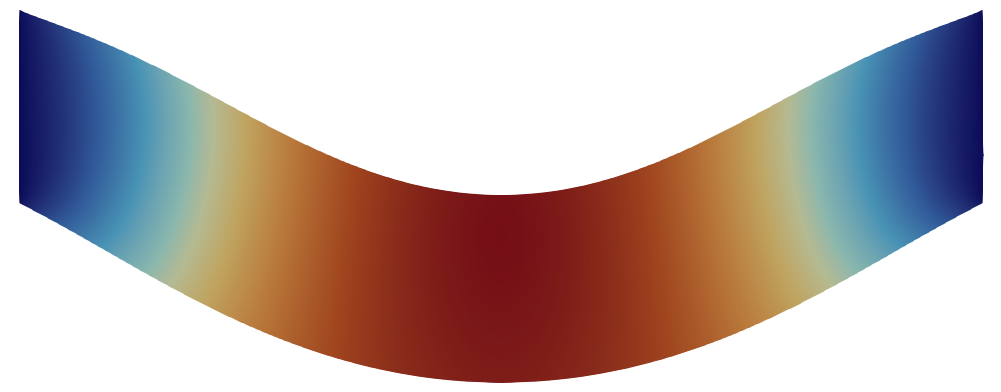
\includegraphics[width=0.65\textwidth]{images/beam-entire.png}};
	\node[anchor=south west,outer sep=0pt] (zoom) at (10.5, -3) {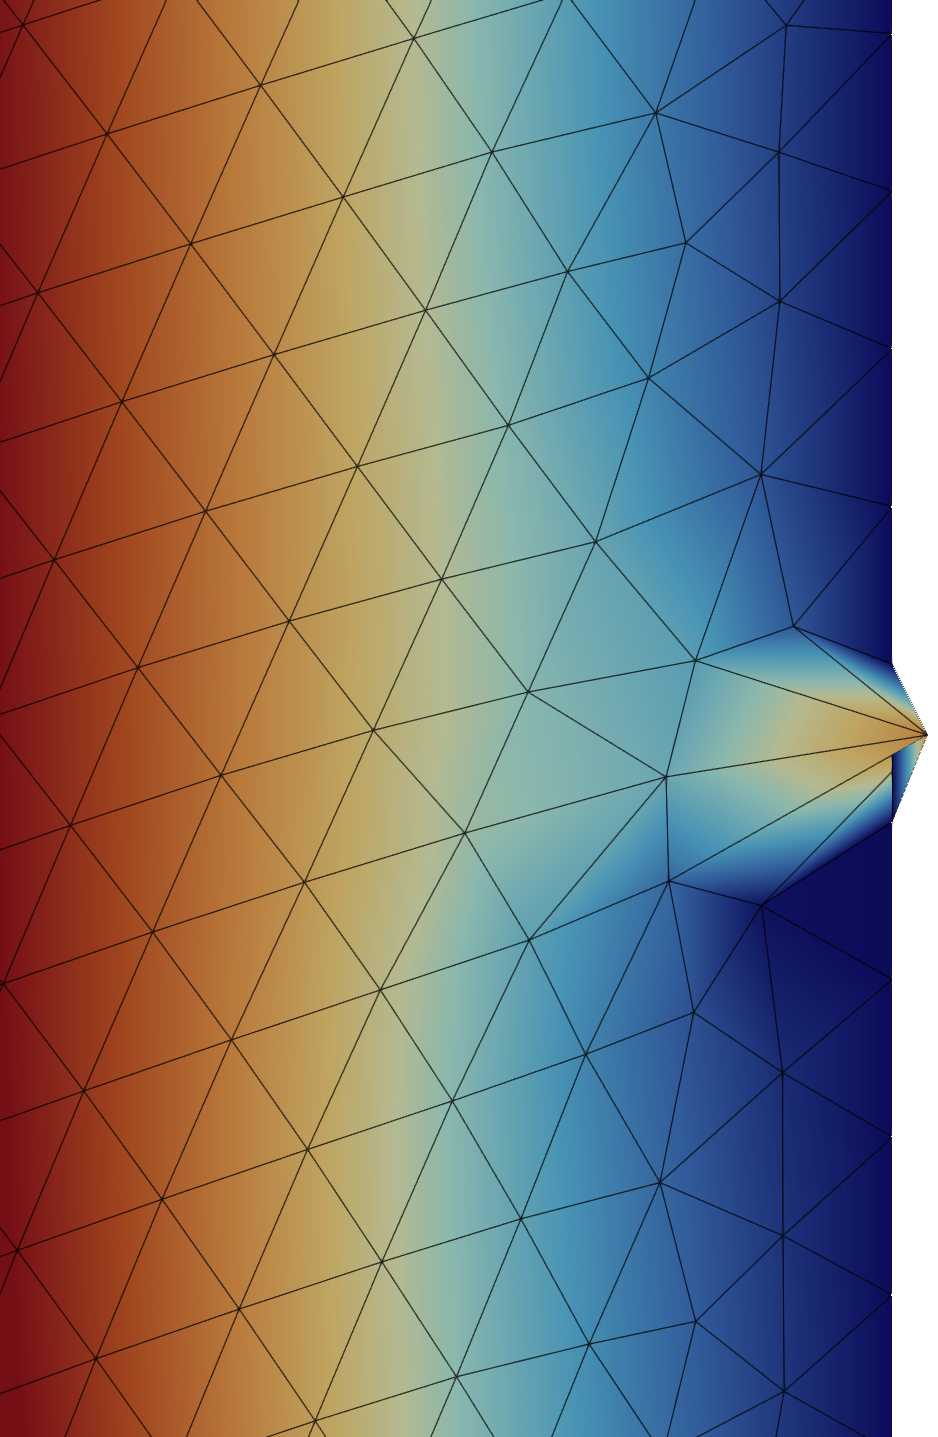
\includegraphics[width=0.15\textwidth]{images/beam-instability.png}};
	\node [draw, thick, minimum size=5mm,outer sep=0pt,red] (a) at ([xshift=-4mm,yshift=4mm]main.east){};

	\draw [thick, dashed] (a.north east) -- ([yshift=-2mm]zoom.north west);
	\draw [thick, dashed] (a.south east) -- ([yshift=2mm]zoom.south west);
\end{tikzpicture}

	}
	\only<2>{
		\begin{tikzpicture}
	\node[anchor=north west] (main) at (0, 0) {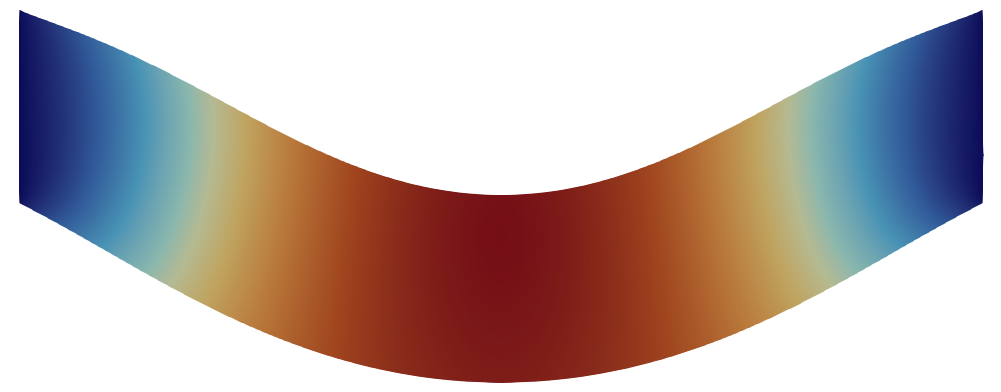
\includegraphics[width=0.65\textwidth]{images/beam-entire.png}};
	\node[anchor=south west,outer sep=0pt] (zoom) at (10.5, -3) {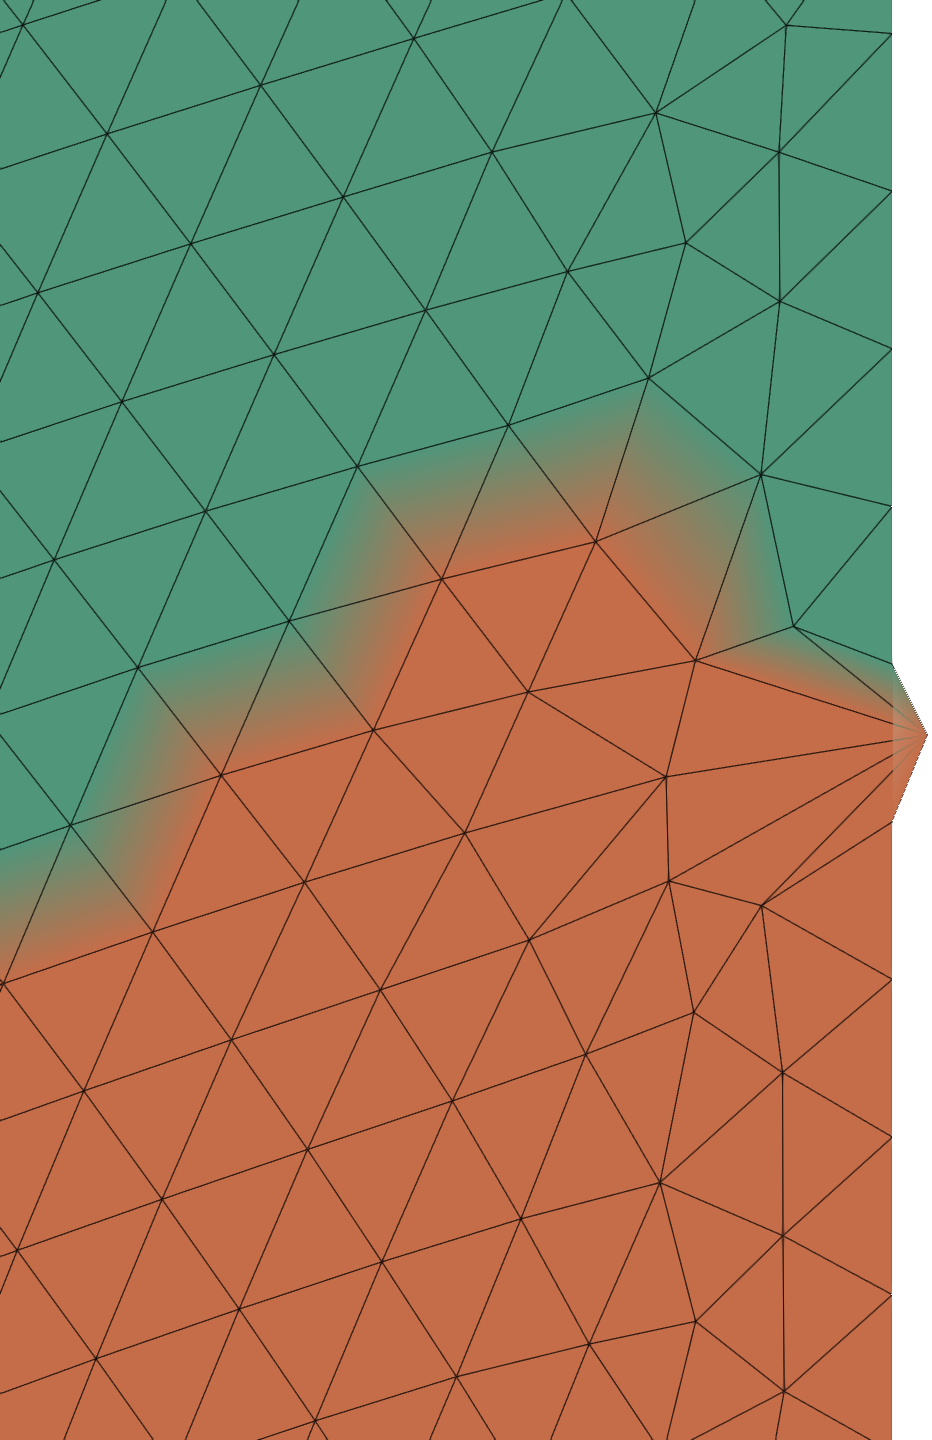
\includegraphics[width=0.15\textwidth]{images/beam-instability-boundary.png}};
	\node [draw, thick, minimum size=5mm,outer sep=0pt,red] (a) at ([xshift=-4mm,yshift=4mm]main.east){};

	\draw [thick, dashed] (a.north east) -- ([yshift=-2mm]zoom.north west);
	\draw [thick, dashed] (a.south east) -- ([yshift=2mm]zoom.south west);
\end{tikzpicture}

	}
\end{frame}

\begin{frame}{Hyperelasticity coarse basis modification}
	\begin{figure}[h!]
		\begin{subfigure}{0.49\textwidth}
			\centering
			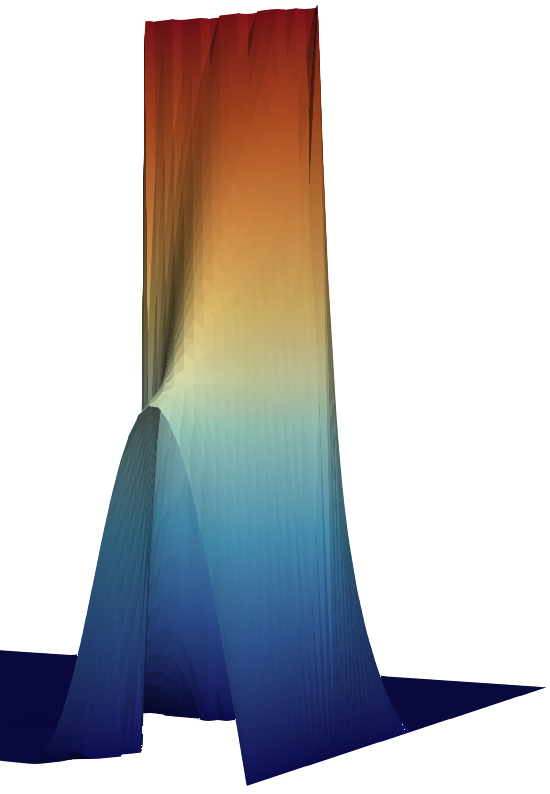
\includegraphics[width=0.7\textwidth,height=0.33\textheight]{images/beam-coarse-basis-1.png}
			\caption{\hspace{-20mm}Side view original}
		\end{subfigure}
		\hfill
		\begin{subfigure}{0.49\textwidth}
			\centering
			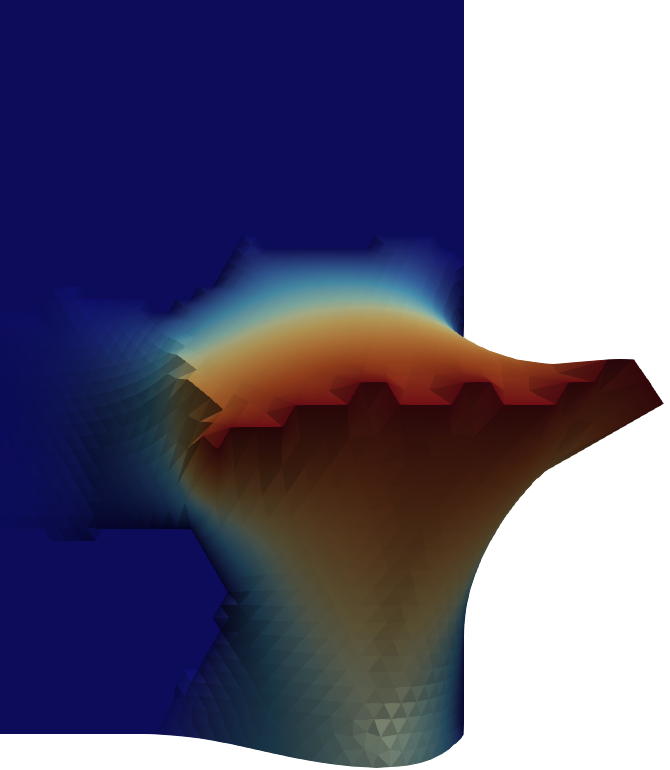
\includegraphics[width=0.7\textwidth,height=0.33\textheight]{images/beam-coarse-basis-2.png}
            \caption{\hspace{-20mm}Top view original}
		\end{subfigure}
		\vfill
		\visible<2->{
			\begin{subfigure}{0.49\textwidth}
				\centering
				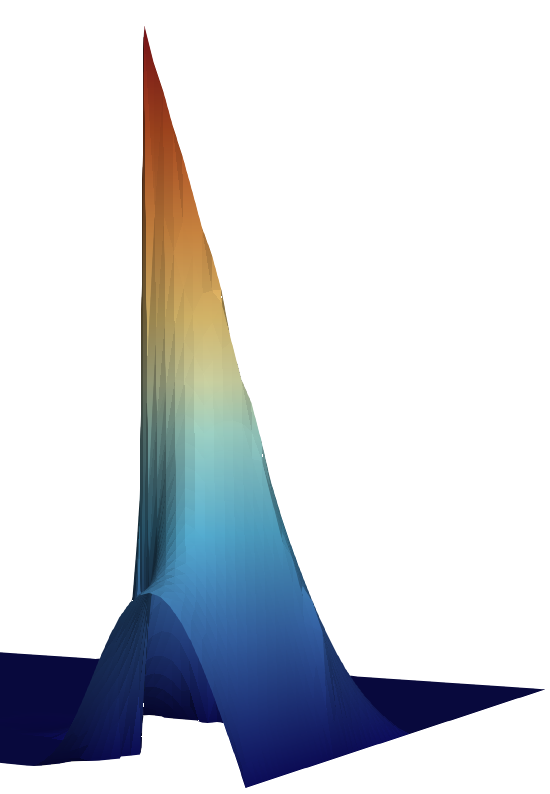
\includegraphics[width=0.7\textwidth,height=0.33\textheight]{images/beam-coarse-basis-3.png}
                \caption{\hspace{-20mm}Side view modified}
			\end{subfigure}
			\hfill
			\begin{subfigure}{0.49\textwidth}
				\centering
				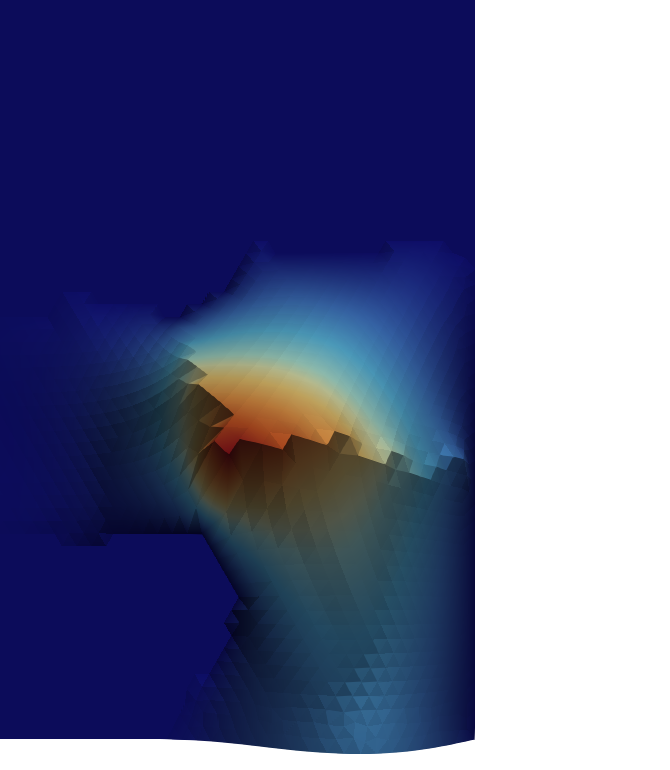
\includegraphics[width=0.7\textwidth,height=0.33\textheight]{images/beam-coarse-basis-4.png}
                \caption{\hspace{-20mm}Top view modified}
			\end{subfigure}
        }
	\end{figure}
\end{frame}

\begin{frame}{Summary}
	\begin{itemize}
		\item The two-level nonlinear Schwarz method is highly sensitive to variations in the coarse space.
		\item It's difficult to tune, e.g., what makes a good coarse space?%: many parameters that have a potentialy significant impact on performance
	\end{itemize}
	\vspace{4mm}
	\begin{center}
		\includegraphics[width=0.6\textwidth]{images/nls.png}\\
		{\tiny \vspace{-2mm}\hspace{-4.7cm}Generated with ChatGPT}
	\end{center}
	% Bottom line: very sensitive to proper tuning, The coarse space does not encode the Re somehow but it's discretisation properties are critical.
\end{frame}



